
\section{Medical Image Synthesis}
\subsection{Background}
\begin{frame}
  \frametitle{Table of Contents}
  \tableofcontents[currentsection]
\end{frame}



%%%%%%%%%%%%%%%%%%%%%%%%%%%%%%%%%%%%%%%%%%%%%%%%%%%%%%%%
{
\paper{
Yi X., Walia E., and Babyn P., "Generative adversarial network in medical imaging: A review." Medical image analysis 58 (2019): 101552.
}

\begin{frame}{Generative adversarial network in medical imaging}{}
      \begin{figure}
        \centering
        \includegraphics[width=1.0\textwidth]{gans-in-medimg-applications/outputs/drawing-v00}
        % \caption{The sonographer-probe-patient control system}
      \end{figure}
\end{frame}
}

%%%%%%%%%%%%%%%%%%%%%%%%%%%%%%%%%%%%%%%%%%%%%%%%%%%%%%%%
{
\paper{
Yi X., Walia E., and Babyn P., "Generative adversarial network in medical imaging: A review." Medical image analysis 58 (2019): 101552.
}

\begin{frame}{Generative adversarial network in medical imaging}{}
      \begin{figure}
        \centering
        \includegraphics[width=1.0\textwidth]{gans-in-medimg-task-modalities-papers/outputs/drawing-v00}
        % \caption{The sonographer-probe-patient control system}
      \end{figure}
\end{frame}
}




\subsection{Methods}

%%%%%%%%%%%%%%%%%%%%%%%%%%%%%%%%%%%%%%%%%%%%%%%%%%%%%%%%
{
\paper{
Yi X., Walia E., and Babyn P., "Generative adversarial network in medical imaging: A review." Medical image analysis 58 (2019): 101552.
}

\begin{frame}{GANs background}
% \BigSizeFont
\begin{itemize}

\item Challenges in optimisitation
    \begin{itemize}
    \item Balance and stabilisation for training of $G$ and $D$, 
    \item Mode collapse (limiting learning to few modes)
    \end{itemize}

\item Varians of GANS
    \begin{itemize}
    \item Varying objective of $D$
    \item Varying objective of $G$
    \item Varying arquitecture
    \end{itemize}

\end{itemize}

\end{frame}
}



%%%%%%%%%%%%%%%%%%%%%%%%%%%%%%%%%%%%%%%%%%%%%%%%%%%%%%%%
{
\paper{
Yi X., Walia E., and Babyn P., "Generative adversarial network in medical imaging: A review." Medical image analysis 58 (2019): 101552.
}

\begin{frame}{Generative adversarial network in medical imaging}{}
      \begin{figure}
        \centering
        \includegraphics[width=1.0\textwidth]{gans-in-medimg-variants/outputs/drawing-v00}
        % \caption{The sonographer-probe-patient control system}
      \end{figure}
\end{frame}
}






\subsection{Applications}

